\documentclass[10pt,a4paper]{article}
\usepackage[a4paper,margin=14mm,top=12mm,bottom=14mm]{geometry}
\usepackage{fontspec}
\setmainfont{Liberation Sans}
\usepackage{polyglossia}
\setdefaultlanguage{french}
\usepackage{amsmath}
\usepackage{xcolor}
\usepackage{graphicx}
\usepackage[most]{tcolorbox}
\usepackage{tabularx,booktabs,array,multirow}
\usepackage{enumitem}
\usepackage{fancyhdr}
\usepackage{lastpage}
\usepackage[hidelinks]{hyperref}
\definecolor{uimm}{HTML}{005677}
\definecolor{cyan}{HTML}{13A2DD}
\definecolor{fond}{HTML}{E6F2FA}
\definecolor{ok}{HTML}{2E7D32}
\definecolor{ko}{HTML}{B3261E}
\definecolor{violet}{HTML}{7B1FA2}
\setlength{\parindent}{0pt}
\setlength{\parskip}{3pt}
\setlist{nosep}
\setlist[itemize]{leftmargin=13pt,label=\textcolor{cyan}{\textbullet}}
\newcommand{\titre}[1]{\vspace{5pt}{\color{uimm}\large\bfseries #1}\par\vspace{-3pt}{\color{cyan}\rule{\linewidth}{1.2pt}}\par\vspace{0pt}}
\tcbset{boite/.style={colback=fond,colframe=uimm,boxrule=0.6pt,arc=2pt,left=6pt,right=6pt,top=4pt,bottom=4pt},
        defi/.style={colback=violet!6,colframe=violet,boxrule=0.8pt,arc=2pt,left=6pt,right=6pt,top=4pt,bottom=4pt,
                     title={\bfseries Défi},coltitle=white,colbacktitle=violet,fonttitle=\small}}
\newcommand{\bandeau}[3]{%
\begin{tcolorbox}[colback=uimm,colframe=uimm,arc=2pt,left=4pt,right=8pt,top=4pt,bottom=4pt]
\begin{minipage}[c]{18mm}\setlength{\fboxsep}{1.2pt}\fcolorbox{white}{white}{
\includegraphics[height=16.5mm]{logo_uimm.jpg}}\end{minipage}\hspace{4mm}%
\begin{minipage}[c]{\dimexpr\linewidth-22mm\relax}\color{white}
{\small #1}\\[1pt]{\LARGE\bfseries #2}\\[2pt]{\large #3}\hfill{\small CQPM Technicien qualité}
\end{minipage}
\end{tcolorbox}}
\newcommand{\reponse}[1][1]{\par\vspace{2pt}{\color{gray!60}\foreach \i in {1,...,#1}{\rule{\linewidth}{0.3pt}\par\vspace{9pt}}}}
\usepackage{pgffor}
\pagestyle{fancy}\fancyhf{}
\renewcommand{\headrulewidth}{0pt}
\newcommand{\pied}[1]{\fancyfoot[L]{\footnotesize\color{uimm}#1}\fancyfoot[R]{\footnotesize\color{uimm}Page \thepage{} sur \pageref{LastPage}}}

\usepackage{tikz}
\usepackage{longtable}
\renewcommand{\bandeau}[3]{%
\begin{tcolorbox}[colback=uimm,colframe=uimm,arc=2pt,left=4pt,right=8pt,top=4pt,bottom=4pt]
\begin{minipage}[c]{18mm}\setlength{\fboxsep}{1.2pt}\fcolorbox{white}{white}{
\includegraphics[height=16.5mm]{logo_uimm.jpg}}\end{minipage}\hspace{4mm}%
\begin{minipage}[c]{\dimexpr\linewidth-22mm\relax}\color{white}
{\small #1}\\[1pt]{\LARGE\bfseries #2}\\[2pt]{\large #3}
\end{minipage}
\end{tcolorbox}}
% en-tête d'une fiche : code, titre, question, bloc, durée, organisation, niveau
\newcommand{\entete}[7]{%
\begin{tcolorbox}[colback=uimm,colframe=uimm,arc=2pt,left=4pt,right=6pt,top=4pt,bottom=4pt]
\begin{minipage}[c]{18mm}\setlength{\fboxsep}{1.2pt}\fcolorbox{white}{white}{
\includegraphics[height=16.5mm]{logo_uimm.jpg}}\end{minipage}\hspace{3mm}%
\begin{minipage}[c]{\dimexpr\linewidth-58mm\relax}\color{white}\raggedright
{\small Base SPC · #4}\\[1pt]{\Large\bfseries #1 · #2}\\[2pt]{\itshape #3}
\end{minipage}\hfill
\begin{minipage}[c]{33mm}\color{white}\small\raggedleft
Durée : \textbf{#5}\\ \textbf{#6}\\ Niveau #7 sur 3
\end{minipage}
\end{tcolorbox}}
\newcommand{\tagE}{{\setlength{\fboxsep}{1.5pt}\colorbox{cyan}{\color{white}\scriptsize\bfseries Ellistat}}}
\newcommand{\tagW}{{\setlength{\fboxsep}{1.5pt}\colorbox{uimm}{\color{white}\scriptsize\bfseries Page web}}}
\tcbset{pred/.style={colback=orange!6,colframe=orange!80!black,boxrule=0.6pt,arc=2pt,left=6pt,right=6pt,top=3pt,bottom=1pt,
                    title={\bfseries Je prédis, avant de commencer},coltitle=white,colbacktitle=orange!80!black,fonttitle=\small},
        retenir/.style={colback=fond,colframe=uimm,boxrule=0.6pt,arc=2pt,left=6pt,right=6pt,top=3pt,bottom=3pt,
                    title={\bfseries À retenir},coltitle=white,colbacktitle=uimm,fonttitle=\small},
        plus/.style={colback=violet!6,colframe=violet,boxrule=0.6pt,arc=2pt,left=6pt,right=6pt,top=3pt,bottom=3pt,
                    title={\bfseries Pour aller plus loin},coltitle=white,colbacktitle=violet,fonttitle=\small},
        act/.style={colback=uimm!10,colframe=uimm,boxrule=0.5pt,arc=2pt,left=5pt,right=5pt,top=2pt,bottom=2pt,before skip=7pt,after skip=3pt},
        verif/.style={colback=orange!6,colframe=orange!80!black,boxrule=0.6pt,arc=2pt,left=6pt,right=6pt,top=3pt,bottom=3pt,
                    title={\bfseries À vérifier sur poste avant la première séance},coltitle=white,colbacktitle=orange!80!black,fonttitle=\small}}
\newcommand{\fichier}[1]{\texttt{\small #1}}
\newcommand{\menu}[1]{\textsf{\textbf{#1}}}
\newcommand{\champ}[1]{\rule{#1}{0.3pt}}

\pied{Base SPC · fiche G5 · Quelle cote pose problème ?}
\begin{document}
\thispagestyle{fancy}
\entete{G5}{Quelle cote pose problème ?}{Sur sept cotes de la plaque, laquelle faut-il corriger en premier ?}{Mallettes GUNT : plaques et arbres}{60 min}{en groupe}{3}
\begin{tcolorbox}[boite]\textbf{Le but.} Mesurer sept cotes sur 20 plaques PT102, calculer le Ppk de chacune, puis classer les cotes de deux façons : par nombre de pièces hors tolérance et par Ppk. Les deux classements ne disent pas la même chose.\par\textbf{Il vous faut.} 20 plaques PT102 numérotées (2 mallettes) · Un pied à coulisse par binôme (avec jauge de profondeur) · Le plan de la plaque (dernière page de la fiche) · Ellistat\end{tcolorbox}
\begin{tcolorbox}[pred]Sur sept cotes, laquelle fera le plus de rebuts ? Laquelle n'en fera aucun mais sera pourtant la plus fragile ?\reponse\end{tcolorbox}
\titre{À faire}
\begin{enumerate}[label=\textcolor{cyan}{\textbf{\arabic*.}},leftmargin=15pt,itemsep=1.5pt]
\item Avec le formateur, vérifier quelles cotes se mesurent proprement avec vos instruments : $a$ (longueur), $d$ (largeur), $m$ (paroi), $n$ et $o$ (largeurs des lamages), $q$ (épaisseur), $r$ (profondeur). Écarter celles qui ne passent pas.
\item Compléter le tableau : limite basse et limite haute de chaque cote d'après le plan (dernière page). Pour $a$ et $m$, aucune tolérance n'est écrite : appliquer la tolérance générale ISO 2768-mK, classe m ($\pm 0{,}3$ pour $a$, $\pm 0{,}2$ pour $m$ ; encadré « Lire le plan GUNT »).
\item Répartir les cotes entre les binômes (deux cotes chacun). Chaque binôme mesure ses cotes sur les 20 plaques et note les valeurs.
\item \tagE\ Réunir toutes les mesures dans une même grille, une colonne par cote. Pour chaque colonne, panneau de colonne, onglet \menu{Informations} : \menu{Nom}, \menu{Nb décimales} 2, \menu{Tolerance min} et \menu{Tolerance max} (comme en E3).
\item \tagE\ \menu{Stats Desc.}, \menu{Détail}, une colonne à la fois : relever moyenne, écart type, Ppk, nombre de plaques hors tolérance et \% hors tolérance attendu.
\item Classer les cotes : (a) par nombre de plaques hors tolérance, du plus grand au plus petit ; (b) par Ppk, du plus petit au plus grand. Tracer le diagramme de Pareto de (a) sur une feuille.
\end{enumerate}
\vspace{3pt}{\renewcommand{\arraystretch}{1.5}\begin{tabularx}{\linewidth}{|l|*{6}{>{\centering\arraybackslash}X|}}\hline
\textbf{Cote et tolérance du dessin} & \textbf{Limite basse} & \textbf{Limite haute} & \textbf{Moyenne} & \textbf{Écart type} & \textbf{Ppk} & \textbf{Hors tol.}\\\hline
a : 105, ISO 2768-mK &  &  &  &  &  & \\\hline
d : 75 +0,3 / 0 &  &  &  &  &  & \\\hline
m : 6,5, ISO 2768-mK &  &  &  &  &  & \\\hline
n : 28 +0,1 / −0,3 &  &  &  &  &  & \\\hline
o : 34 ± 0,1 &  &  &  &  &  & \\\hline
q : 19 0 / −0,3 &  &  &  &  &  & \\\hline
r : 16 0 / −0,3 &  &  &  &  &  & \\\hline
\end{tabularx}}\par
\newpage
\titre{J'observe, je décide}
\begin{enumerate}[label=\textcolor{cyan}{\textbf{Q\arabic*.}},leftmargin=22pt]
\item Quelle cote produit le plus de pièces hors tolérance ? Quelle part du total des rebuts ?\reponse[1]
\item Quelle cote n'a aucun rebut mais un Ppk inférieur à 1 ? Combien de pièces hors tolérance Ellistat annonce-t-il pour la population ?\reponse[2]
\item Les deux classements donnent-ils le même ordre ? Lequel prévient le mieux les rebuts de demain ?\reponse[2]
\item Pour les deux cotes les plus critiques, comparez la moyenne au milieu de la tolérance : de combien décaler ? Cela suffit-il (comparez Pp à 1,33) ?\reponse[2]
\item Pour la cote $o$ ($T = 0{,}2$ mm), la mesure elle-même est-elle assez fine ? (règle de M1)\reponse[1]
\end{enumerate}
\begin{tcolorbox}[retenir]Compter les rebuts regarde le passé. Le Ppk regarde ce que le procédé va produire. Une cote sans rebut peut être la plus fragile.\end{tcolorbox}
\providecommand{\carre}{\fbox{\rule{0pt}{1.1ex}\rule{1.1ex}{0pt}}}
\begin{tcolorbox}[boite,left=5pt,right=5pt,top=3pt,bottom=3pt]\footnotesize
\textbf{\color{uimm}Lire le plan GUNT (dernière page).} Le cartouche du plan est écrit en allemand et en anglais. À la ligne « Allgemeintoleranzen / General tolerance », on lit \textbf{ISO 2768-mK}. Cela veut dire : toute cote \textbf{sans écart écrit} a la tolérance générale de la classe \textbf{m} (« medium »), donnée par le tableau ci-dessous. Une cote \textbf{avec un écart écrit} garde cet écart, et la tolérance générale ne s'applique pas. Limite haute = nominal + écart supérieur. Limite basse = nominal + écart inférieur. \O\ : diamètre. \carre{} : carré, on lit son côté. « A-A », « B-B » : coupes. Les symboles d'état de surface et d'arêtes, en bas à droite, ne servent pas dans cette fiche.
\par\vspace{6pt}\noindent\renewcommand{\arraystretch}{1.2}\setlength{\tabcolsep}{4pt}
\begin{tabular}{|l|c|c|c|c|c|}\hline
\textbf{Dimension nominale (mm)} & 0,5 à 3 & au-delà de 3 à 6 & au-delà de 6 à 30 & au-delà de 30 à 120 & au-delà de 120 à 400\\\hline
\textbf{Écart de la classe m (mm)} & $\pm 0{,}1$ & $\pm 0{,}1$ & $\pm 0{,}2$ & $\pm 0{,}3$ & $\pm 0{,}5$\\\hline
\end{tabular}
\par\vspace{1pt}{\scriptsize Source : ISO 2768-1:1989, tolérances générales des dimensions linéaires, reprises dans la fiche GUNT « PT105f Tolérances ».}
\par\vspace{4pt}\textbf{Les cotes de cette fiche}\par\vspace{2pt}
\begin{tabularx}{\linewidth}{|c|>{\raggedright\arraybackslash}X|>{\raggedright\arraybackslash}X|}\hline
\textbf{Cote} & \textbf{Ce que le plan écrit} & \textbf{Écart à utiliser}\\\hline
$a$ & 105, aucun écart écrit & classe m, plage 30 à 120 : $\pm 0{,}3$ \\\hline
$d$ & 75 avec $+0{,}3$ et $-0{,}0$ & écrit sur le plan : $+0{,}3$ et $0$ \\\hline
$m$ & 6,5, aucun écart écrit & classe m, plage au-delà de 6 jusqu'à 30 : $\pm 0{,}2$ \\\hline
$n$ & \hspace{2pt}\carre{}\ 28, avec $+0{,}1$ et $-0{,}3$ & écrit sur le plan : $+0{,}1$ et $-0{,}3$ \\\hline
$o$ & \hspace{2pt}\carre{}\ 34, avec $+0{,}1$ et $-0{,}1$ & écrit sur le plan : $+0{,}1$ et $-0{,}1$ \\\hline
$q$ & 19 avec $+0{,}0$ et $-0{,}3$ & écrit sur le plan : $+0{,}0$ et $-0{,}3$ \\\hline
$r$ & 16 avec $+0{,}0$ et $-0{,}3$ & écrit sur le plan : $+0{,}0$ et $-0{,}3$ \\\hline
\end{tabularx}
\end{tcolorbox}
\vfill{\footnotesize\color{uimm}\textbf{Ressources de la base :} Données de secours : \href{https://sjaubert.github.io/000_OI/SPC/Pages/Donnees_a_copier.html\#cotes7}{\nolinkurl{https://sjaubert.github.io/000_OI/SPC/Pages/Donnees_a_copier.html}}}
\newpage
\titre{Plan de la plaque PT102}
{\small Pour lire ce plan et ses tolérances, voir l'encadré « Lire le plan GUNT » de la page précédente.\par}\vspace{2pt}
\begin{center}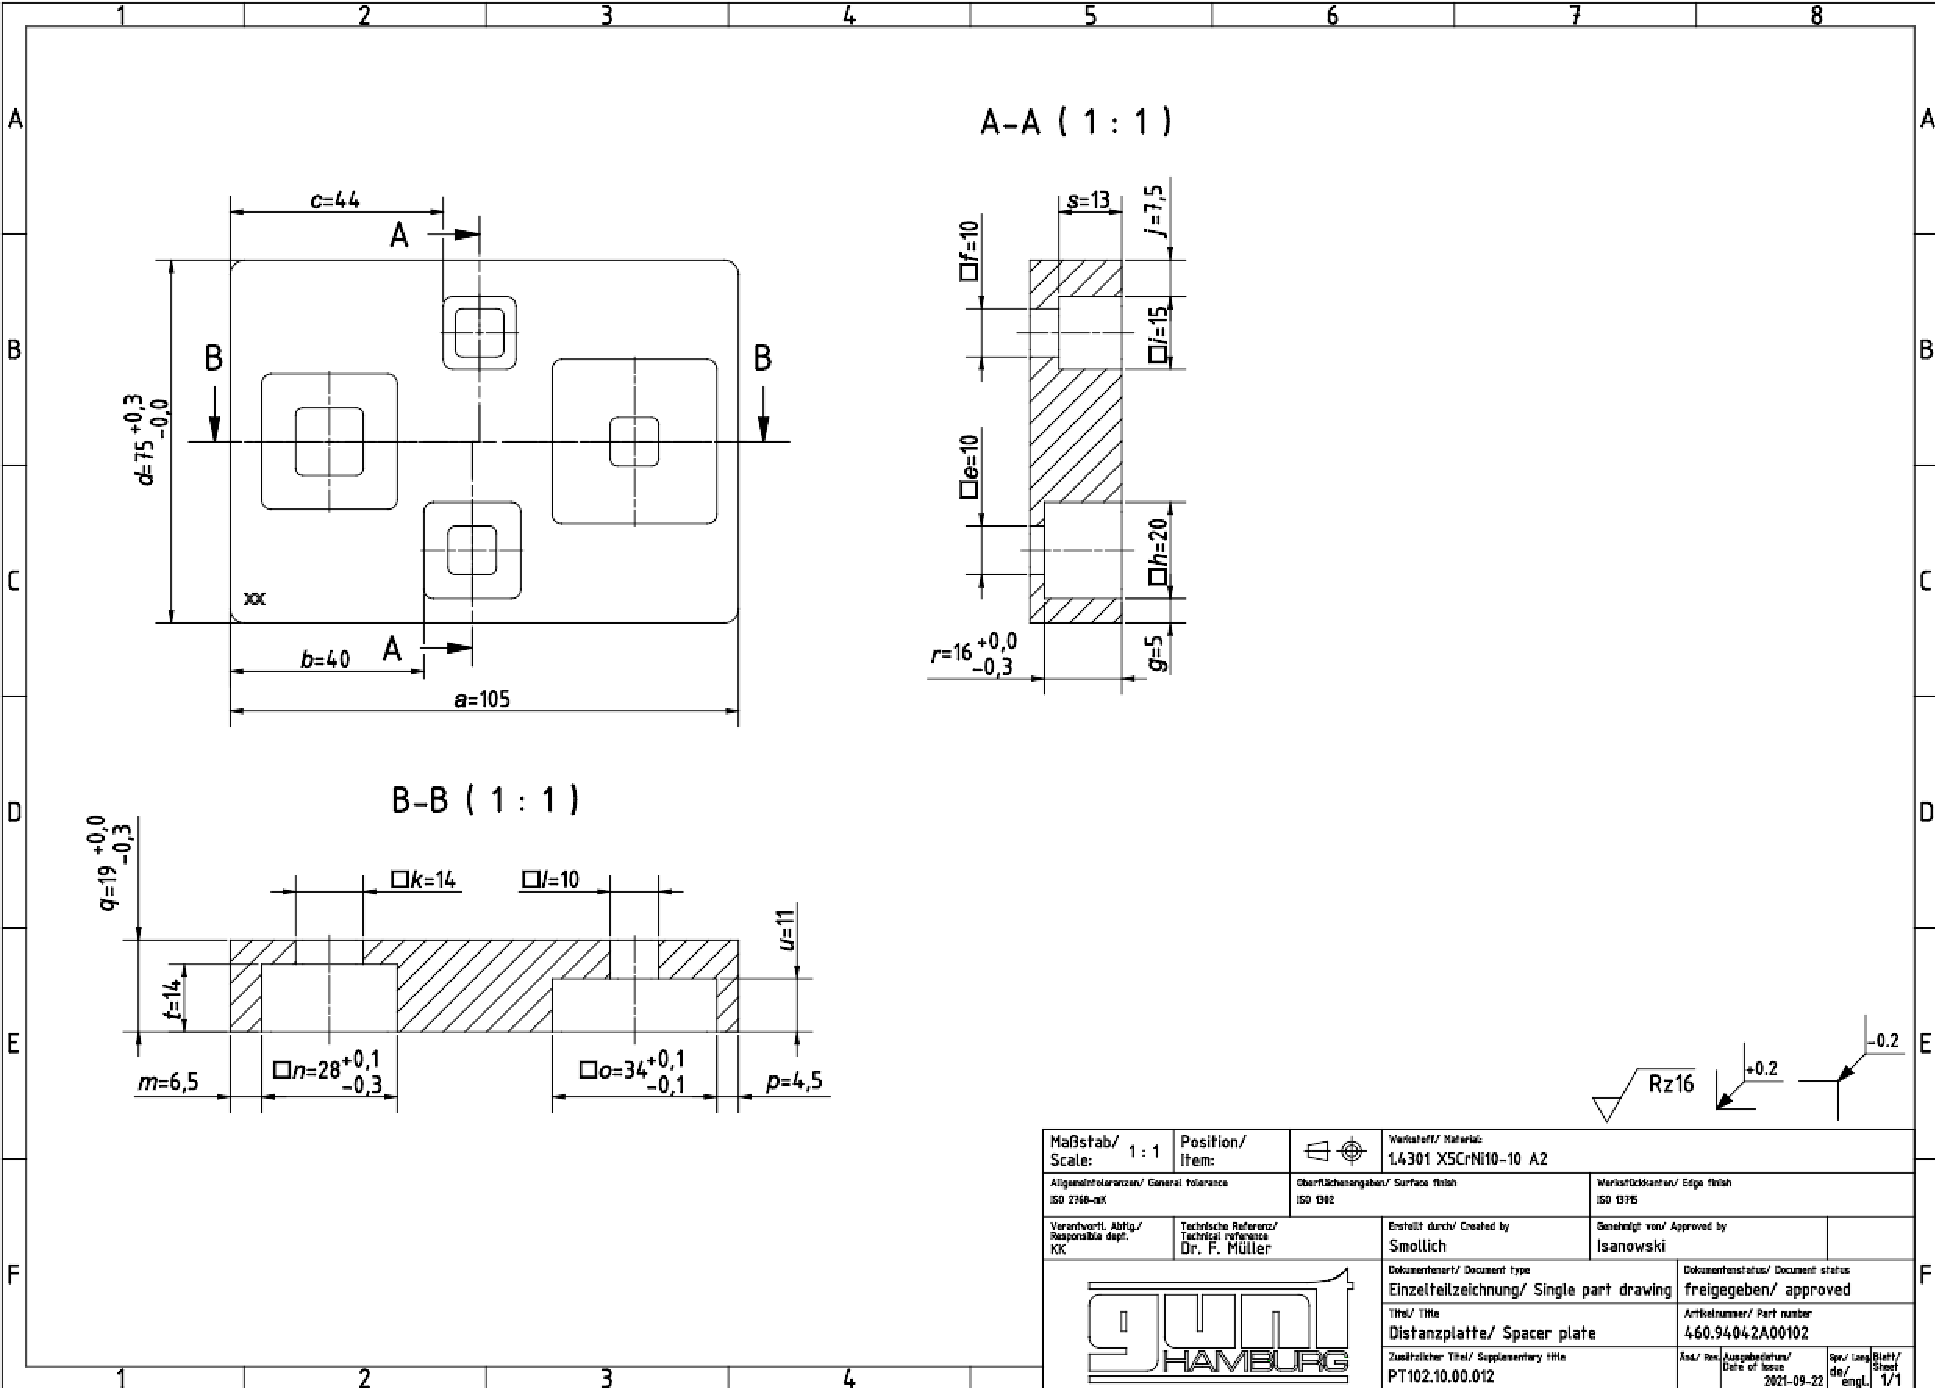
\includegraphics[width=0.90\textheight,height=0.97\linewidth,keepaspectratio,angle=90]{plan_plaque_PT102.pdf}\end{center}
\vfill{\footnotesize\color{uimm}Plan : GUNT Hamburg, Distanzplatte (plaque d'écartement), dessin PT102.10.00.012.}
\end{document}